% generate data and check both pieces of code to confirm that they work; get runtimes and put in table and calculate average runtimes for different input sizes and show how they differ (use desmos graph to determine which input sizes create largest possible divergence between runtimes of cubic, quadratic, and linear algorithms - possible show desmos graph after data to show divergence of both graphs)

% \begin{figure}
  % \caption{Comparison of Complexities}
  % \centering
    % 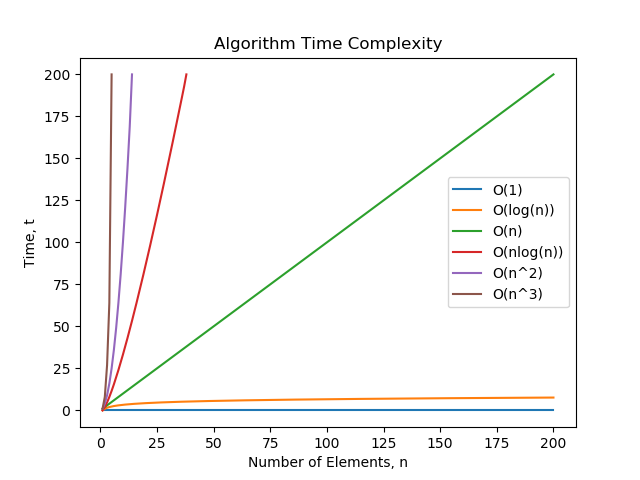
\includegraphics[width = 175mm]{big-o-notation-algorithm-complexity-non-weighted.png}~\cite{Complexity}
% \end{figure}

% \bibliography{sources.bib}
% \bibliographystyle{siam}

